In this section, we explore some applications of community detection. We will start with the simple example of Zachary's Karate Club and build up to more complicated examples.

\subsection{Zachary's Karate Club}
To add more to the context already introduced in Section \ref{sec:Social Networks}, the karate club that Zachary studied had two main leaders who are referred to in the paper as ``Mr Hi" and ``John A". Due to some inter-personal politics, members of the club ended up becoming part of a faction that was politically aligned with one of the primary leaders. Zachary collected all the data relating to this including information on how often any two members of the group interacted and which leader they were factionally affiliated with. Using this data, Zachary built a model that knew how much any two particular members interacted, but no knowledge of their factional affiliations. After developing this model, Zachary was interested in the following two hypotheses:

\begin{enumerate}
    \item Using community detection, can we predict the political affiliation of any member of the club pre-fission,
    \item Using community detection, can we predict which club any member will join after the split.
\end{enumerate}

Zachary's chose to model this problem as a network flow problem so that he could use the \emph{max-flow min-cut theorem} and the \emph{Ford-Fulkerson algorithm}\cite{ford_fulkerson_1956} to test his hypotheses. The max-flow min-cut theorem states that the maximum flow across a network is equal to the capacity of the minimum cut and the Ford-Fulkerson algorithm is a deterministic method for finding the minimum cut. Using this model we can rephrase the above two hypotheses:

\begin{enumerate}
    \item The minimum cut of the network should separate those factionally affiliated with Mr Hi from those factionally affiliated with John A.
    \item The minimum cut of the network should separate those who choose to join Mr Hi's club after the split from those who chose to join John A's club after the split.
\end{enumerate}

After running the Ford-Fulkerson algorithm on the data, Zachary achieved results that correctly predicted 34 out of 34 factoin memberships and 33 out of 34 club memberships with the notable exception being individual number 9 who reportedly joined Mr Hi's club so as not to miss out on a black belt which they would have had to give up on if they'd joined John A's group. Figure \ref{fig:zachary_results} shows Zachary's full results.

\begin{figure}
    \begin{center}
        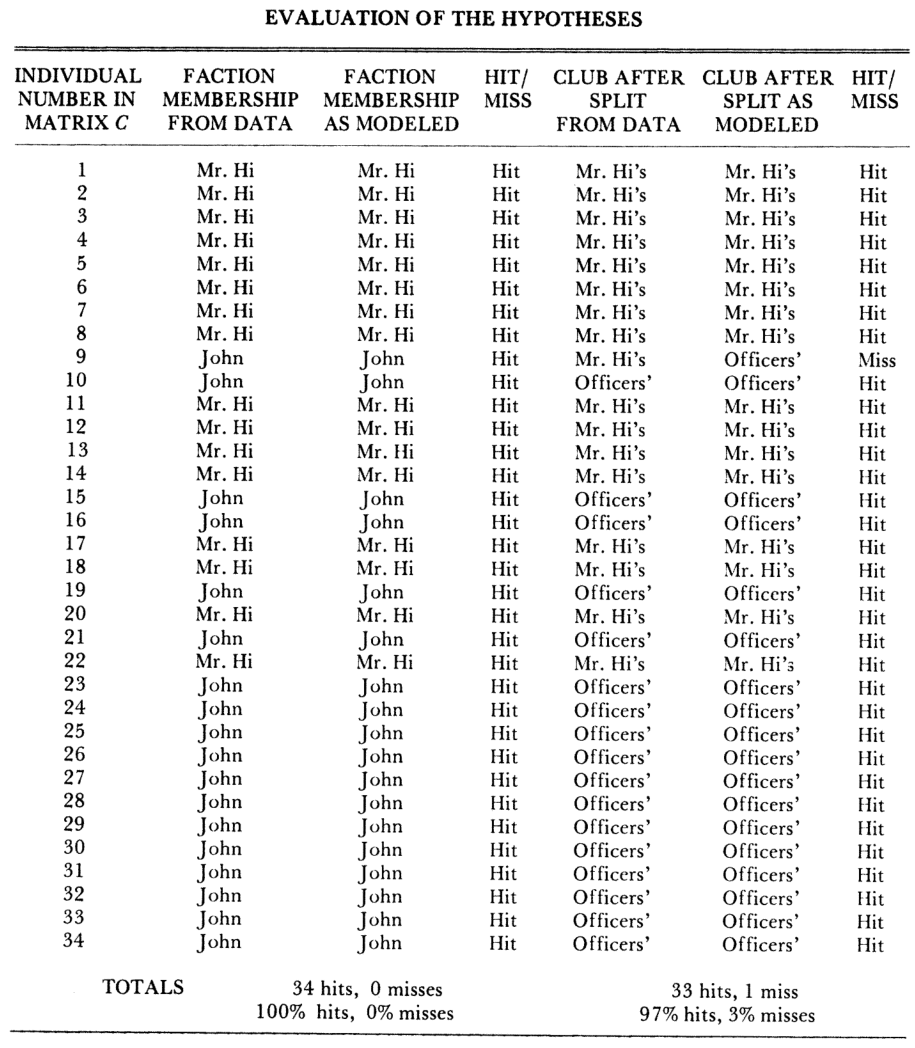
\includegraphics[width=0.95\textwidth]{img/zachary_results}
    \end{center}
    \caption{The full results from Zachary's investigation into using the Ford-Fulkerson minimum-cut algorithm to predict social and political alignments.\cite{konect:ucidata-zachary}}
    \label{fig:zachary_results}
\end{figure}


\todo[backgroundcolor=red]{SEC: Applications of Community Detection}
\todo[backgroundcolor=red]{SEC: Figure out an interesting thing to write some of my own code for}
